%!TEX root = ./template-skripsi.tex
%-------------------------------------------------------------------------------
%                            	BAB IV
%               		KESIMPULAN DAN SARAN
%-------------------------------------------------------------------------------

\chapter{HASIL DAN PEMBAHASAN}

\section{Pengolahan data citra input}
Langkah pertama dalam pengolahan data citra input adalah Proses konversi citra luka RGB menjadi citra luka \emph{grayscale}. Proses konversi citra luka menjadi citra luka \emph{grayscale} dilakukan menggunakan bahasa pemrograman \emph{python} dengan bantuan \emph{library scikit-image}, \emph{library} ini dipilih karena fungsi yang digunakan sama dengan metode \emph{luminosity} di persamaan \ref{luminosity} \citep{rgb2gray}. berikut \emph{source code} nya:
\begin{figure}[H]
	\begin{lstlisting}[language=Python, basicstyle=\tiny]
		img = imread("some_image.jpg")
		img_gray = rgb2gray(img)
	\end{lstlisting}
	\caption{\emph{source code} konversi citra RGB ke \emph{grayscale}}
	\label{Gambar:snap_grayscale}
\end{figure}
fungsi \texttt{imread} dan \texttt{rgb2gray} di-\emph{import} dari \emph{library} \texttt{skimage.io} dan \texttt{skimage.color} yang masing-masing fungsinya adalah untuk membaca dan melakukan konversi citra RGB ke citra \emph{grayscale}. Data citra \emph{grayscale} disimpan kedalam variabel \texttt{img\_gray}. Rincian hasil dari proses ini tersedia di bagian \textbf{lampiran B}.


\section{Deteksi keliling luka menggunakan \emph{active contour} (\emph{snake})}
Proses deteksi keliling luka menggunakan \emph{snake} versi asli \emph{integer} dan metode \emph{snake} yang ditambahkan interpolasi yang datanya berupa nilai \emph{float}. Berikut tahapannya:

\subsection{Inisialisasi kurva awal}
Rincian hasil dari proses ini tersedia di bagian \emph{lampiran C dan D}. Berikut \emph{source code} yang bekerja dengan baik untuk inisialisasi kurva awal:
\begin{figure}[H]
	\begin{lstlisting}[language=Python, basicstyle=\tiny]
		theta = np.linspace(0, 2*np.pi, num_of_sample)
		r = cr + rad*np.sin(theta)
		c = cc + rad*np.cos(s)
		snake_init = np.array([r, c]).T
		
		snake_xy = snake_init[:, ::-1].astype(int)
		x = snake_xy[:, 0]
		y = snake_xy[:, 1]
	\end{lstlisting}
	\caption{\emph{source code} inisialisasi kurva lingkaran versi \emph{integer}}
	\label{Gambar:circle_integer}
\end{figure}
\begin{figure}[H]
	\begin{lstlisting}[language=Python, basicstyle=\tiny]
		theta = np.linspace(0, 2*np.pi, num_of_sample)
		r = cr + rad*np.sin(theta)
		c = cc + rad*np.cos(theta)
		snake = np.array([r, c]).T
		
		snake_xy = snake[:, ::-1]
		x = snake_xy[:, 0].astype(float)
		y = snake_xy[:, 1].astype(float)
	\end{lstlisting}
	\caption{\emph{source code} inisialisasi kurva lingkaran versi interpolasi}
	\label{Gambar:circle_float}
\end{figure}
Potongan kode (\ref{Gambar:circle_integer}) dan (\ref{Gambar:circle_float}) diimplementasi berdasarkan algoritma pembuatan lingkaran menggunakan bentuk parametrik (\emph{parametric form}) lingkaran (\ref{Gambar:algo_circle}). \texttt{theta} yang didapatkan menggunakan fungsi \texttt{np.linspace} milik \texttt{numpy} menghasilkan \emph{array} dengan \emph{step} yang sama dan nilai-nilai di dalam \texttt{theta} berjumlah \texttt{num\_of\_sample} dengan \emph{range} $0$ sampai $2 \pi$, \texttt{cc} dan \texttt{cr} adalah titik tengah lingkaran dan\texttt{rad} adalah jari-jari. Kurva awal \emph{snake} ini disimpan kedalam variabel \texttt{snake\_xy}.

\begin{comment}
	Metode lain dalam inisialisasi kurva adalah dengan cara manual. Ketika metode ini sudah masuk ke penerapan untuk \emph{assesment} luka, inisialisasi secara manual yang dilakukan perawat luka adalah salah satu opsi proses deteksi keliling luka menggunakan \emph{snake}. Selain itu metode \emph{snake} cenderung menghasilkan hasil yang baik jika inisialisasi kurva awal ditempatkan di dekat target\citep{guo2013review:20}. Penulis menggunakan fitur \emph{draw path} milih GIMP dalam proses inisialisasi kurva secara manual dan rinciannya terdapat pada bagian \textbf{Rancangan eksperimen}. Namun saat implementasi ke program, penulis menemukan kendala ketika membaca kurva yang penulis buat menggunakan GIMP, koordinat dari kurva yang terinisialisasi manual terurut secara baris dan kolom sementara itu, dibutuhkan keterurutan secara ketetanggaan.
\end{comment}



\subsection{Energi internal}
\emph{output} dari energi internal adalah sebuah matriks yang elemennya dipengaruhi oleh parameter $\alpha$, $\beta$, dan \emph{time step} seperti pada matriks (\ref{matriks_m}). Berikut \emph{source code} yang bekerja dengan baik untuk menghasilkan matriks energi internal:
\begin{figure}[H]
	\begin{lstlisting}[language=Python, basicstyle=\tiny]
		a = beta
		b = -(4*beta + alpha)
		c = 6*beta + 2*alpha
		
		eye_n = np.eye(n, dtype=float)
		c_axis = c * eye_n
		b_axis = b * ( np.roll(eye_n, -1, axis=0) + np.roll(eye_n, -1, axis=1) )
		a_axis = a * ( np.roll(eye_n, -2, axis=0) + np.roll(eye_n, -2, axis=1) )
		A = c_axis + b_axis + a_axis
		
		inv = np.linalg.inv(A + gamma * eye_n)
	\end{lstlisting}
	\caption{\emph{source code} untuk menghasilkan energi internal}
	\label{code:energy_internal}
\end{figure}
Penulis mengimplementasi (\ref{matriks_m}) dengan memanggil beberapa fungsi dari \emph{library numpy}. Fungsi \texttt{np.eye(n)} menghasilkan matriks identitas dengan ukuran \texttt{n x n}. \texttt{np.roll} digunakan untuk mengubah nilai pada diagonal tertentu pada suatu matriks. \texttt{np.linalg.inv} digunakan untuk menghitung invers matriks. Variabel \texttt{a} dan \texttt{b} masing masing mewakili $p$ dan $q$ pada matriks (\ref{matriks_m}). \texttt{eye\_n} adalah matriks identitas dengan ukuran \texttt{n x n} di mana \texttt{n} adalah panjang dari vektor kurva \emph{snake}. \texttt{a\_axis}, \texttt{b\_axis}, dan \texttt{c\_axis} masing-masing adalah elemen matriks yang mengisi $p$, $q$, dan $r$ pada matriks (\ref{matriks_m}). \texttt{A + gamma * eye\_n} adalah cara untuk membuat elemen-elemen pada matriks sesuai dengan $p$, $q$, dan $r$ pada matriks (\ref{matriks_m}). Matriks energi internal kemudian dihitung inversnya dan invers dari matriks tersebut disimpan kedalam variabel \texttt{inv} untuk digunakan pada persamaan update kurva \emph{snake}. Parameter $\alpha$, $\beta$, dan \emph{time step} untuk setiap data tersedia di bagian \emph{lampiran C dan D}

\subsection{Energi eksternal}
Untuk versi \emph{integer} energi eksternal menggunakan persamaan (\ref{eext2}). Untuk versi interpolasi yang dipilih adalah persamaan \ref{eext4}, kemudian persamaan \ref{eext4} diproses lagi menggunakan gradien Sobel untuk mendapatkan peta tepi dari citra luka. Berikut \emph{source code} yang bekerja dengan baik untuk menghasilkan energi eksternal:
\begin{figure}[H]
	\begin{lstlisting}[language=Python, basicstyle=\tiny]
		ext = gaussian(im_gray, sigma)
		ext = sobel(ext)
		ext = -ext**2
	\end{lstlisting}
	\caption{\emph{source code} energi eksternal untuk \emph{snake} versi \emph{integer}}
	\label{Gambar:external_int}
\end{figure}
\begin{figure}[H]
	\begin{lstlisting}[language=Python, basicstyle=\tiny]
		ext = gaussian(im_gray, sigma)
		ext = img_as_float(ext)
		ext = ext.astype(float, copy=False)
		ext = sobel(ext)
	\end{lstlisting}
	\caption{\emph{source code} energi eksternal untuk \emph{snake} versi interpolasi}
	\label{Gambar:external_float}
\end{figure}
Penulis mengimplementasi energi eksternal dengan memanggil beberapa fungsi dari \emph{library scikit-image}. Fungsi \texttt{gaussian} menghasilkan citra gaussian $G_{\sigma} (x,y) * I(x,y)$ dengan standar deviasi \texttt{sigma}, sedangkan yang dihasilkan fungsi \texttt{sobel} adalah besar gradien sobel, sesuai dengan persamaan (\ref{sobel_mag}). Energi eksternal disimpan kedalam variabel \texttt{ext}. Rincian hasil dari proses ini tersedia di bagian \emph{lampiran C dan D}.

\subsection{Proses update intersi kurva}
Berikut \emph{source code} yang bekerja dengan baik untuk proses update iterasi kurva atau dapat disebut \emph{snake evolution}:
\begin{figure}[H]
	\begin{lstlisting}[language=Python, basicstyle=\tiny]
		# potential force
		gy, gx = np.gradient(ext)
		
		xt = np.copy(x)
		yt = np.copy(y)
		
		max_num_iter=n
		for i in range(max_iter):
			fx = np.array([])
			fy = np.array([])
			
			for i in range(n):
				fx = np.append(fx, gx[yt[i]] [xt[i]] )
				fy = np.append(fy, gy[yt[i]] [xt[i]] )
			
			xn = np.dot(inv, xt + gamma * fx) # acton, ivins equation
			yn = np.dot(inv, yt + gamma * fy)
			
			xt = np.round(xn).astype(int)
			yt = np.round(yn).astype(int)
		
		snake_final = np.array([xt, yt]).T
	\end{lstlisting}
	\caption{\emph{source code} proses update iterasi kurva versi \emph{integer}}
	\label{code:snake_evol_int}
\end{figure}
\begin{figure}[H]
	\begin{lstlisting}[language=Python, basicstyle=\tiny]
		# potential force
		gy, gx = np.gradient(ext)
		
		# Interpolate for smoothness
		intp1 = RectBivariateSpline(np.arange(gx.shape[1]),
									np.arange(gx.shape[0]),
									gx.T, kx=2, ky=2, s=0)
		
		intp2 = RectBivariateSpline(np.arange(gy.shape[1]),
									np.arange(gy.shape[0]),
									gy.T, kx=2, ky=2, s=0)
		
		
		# deform snake
		max_num_iter=n
		max_px_move=1.0
		
		xt = np.copy(x)
		yt = np.copy(y)
		
		for i in range(max_num_iter):
			# fx & fy
			fx = intp1(xt, yt, dx=0, grid=False).astype(float, copy=False)
			fy = intp2(xt, yt, dy=0, grid=False).astype(float, copy=False)
		
			# skimage equation
			xn = np.dot(inv, gamma * xt + fx)
			yn = np.dot(inv, gamma * yt + fy)
		
			# Movements are capped to max_px_move per iteration. skimage
			dx = max_px_move * np.tanh(xn - xt)
			dy = max_px_move * np.tanh(yn - yt)
		
			xt += dx
			yt += dy
		
		snake_final = np.array([xt, yt]).T
	\end{lstlisting}
	\caption{\emph{source code} proses update iterasi kurva versi interpolasi}
	\label{code:snake_evol_float}
\end{figure}
Metode \emph{snake} versi \emph{integer} dan interpolasi memakai metode gradien arah \emph{direction} untuk mendapatkan turunan pertama citra yang akan digunakan untuk persamaan (\ref{fx_eq}) dan (\ref{fy_eq}). Gradien \emph{direction} $x$ dan $y$ didapat dengan memanggil \texttt{np.gradient} dan disimpan kedalam variabel \texttt{gx} dan \texttt{gy}.

Proses iterasi dilakukan sebanyak \texttt{max\_num\_iter} kali dan yang dilakukan adalah mengupdate nilai \texttt{fx} dan \texttt{fy}. Untuk versi \emph{integer} nilai \texttt{fx} dan \texttt{fy} dapat dihitung secara langsung karena nilainya tersedia di dalam \texttt{gx} dan \texttt{gy} sedangkan untuk versi interpolasi nilainya harus didapatkan melalui proses interpolasi. 

Bentuk kurva \emph{snake} untuk setiap iterasi terdiri dari pasangan koordinat dengan nilai \emph{float}, hal ini menimbulkan masalah pada operasi \emph{finding contour} di setiap iterasi yang menghasilkan koordinat bilangan \emph{float}. Kurva harus diletakkan di atas citra yang menyebabkan terjadi \emph{missing value} pada kurva jika nilai koordinatnya terdiri dari nilai \emph{float}. 
\begin{figure}[H]
	\centering
	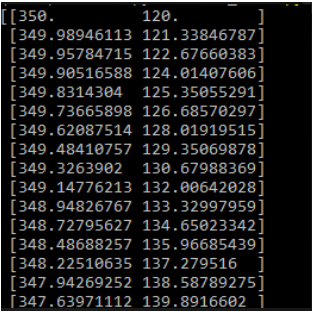
\includegraphics[width=0.5\textwidth]{gambar/curve_vector}
	\caption{Bentuk kurva \emph{snake} terdiri dari pasangan koordinat dengan nilai \emph{float} }
	\label{Gambar:snake_float}
\end{figure}
Untuk mengatasi masalah ini, pada \emph{snake} versi integer dilakukan pembulatan (integer) terhadap kurva.
%Untuk \emph{snake} versi interpolasi dilakukan proses interpolasi yang mana hal ini diperlukan agar bentuk kurva \emph{snake} tetap terdiri dari pasangan koordinat dengan nilai \emph{float}.
Selanjutnya untuk versi interpolasi, peneliti melakukan \emph{tracing} terhadap metode \emph{snake} yang ada di \emph{library scikit-image} dan menemukan sesuatu pada \emph{library} tersebut terdapat modifikasi dari \emph{snake} integer dengan menambahkan interpolasi, sisanya dihipotesiskan sebagai \emph{code minor}. Kontribusi terbesar pada penelitian ini terdapat pada penemuan bahwa interpolasi dibutuhkan untuk menjalankan \emph{snake}. 

Proses interpolasi yang dilakukan \emph{library scikit-image} adalah dengan memanggil \emph{Class} \texttt{RectBivariateSpline} \citep{acm}. \emph{Class} ini menggunakan pendekatan \emph{bivariate spline} di atas \emph{rectangular mesh}, dalam hal ini adalah citra (matriks). \texttt{RectBivariateSpline} dapat digunakan untuk interpolasi data \citep{rbs}. Proses interpolasi yang dilakukan \emph{library scikit-image} dapat dianggap dalam langkah \emph{preprocessing} terhadap citra asli yang mana pengaruhnya adalah arah tepinya semakin jelas dibanding dengan citra asli.
\begin{figure}[H]
	\centering
	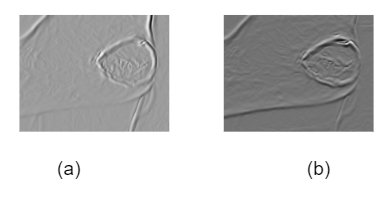
\includegraphics[width=1\textwidth]{gambar/compare_ori_interp}
	\caption{komparasi gradien citra arah (\emph{direction}) $y$ (\texttt{gy}). (a) citra asli (b) citra hasil interpolasi}
	\label{Gambar:compare_ori_interp}
\end{figure}
Proses untuk mendapatkan nilai \texttt{fx} dan \texttt{fy} pada \emph{snake} versi interpolasi adalah dengan menggunakan \emph{class} \texttt{RectBivariateSpline} milik \texttt{scipy} \citep{rbs}. Dengan memanggil metode \texttt{RectBivariateSpline} kita dapat mendapatkan nilai \texttt{fx} dan \texttt{fy} terhadap elemen kurva yang berupa bilangan \emph{float}. Sayangnya pada saat melakukan penelitian penulis tidak menemukan algoritma bagaimana cara mendapatkan nilai \texttt{fx} dan \texttt{fy} menggunakan \texttt{RectBivariateSpline} karena \emph{source code} milik \emph{scipy} sangat kompleks.

Selanjutnya untuk proses update kurva versi \emph{integer} perhitungannya dapat menggunakan persamaan (\ref{implicit_x}) dan (\ref{implicit_y}), sedangkan pada versi interpolasi penulis menggunakan persamaan milik \emph{skimage} \citep{acm} karena jika menggunakan persamaan (\ref{implicit_x}) dan (\ref{implicit_y}) kurva tidak mau bergerak. Persamaan ini memodifikasi sedikit dari persamaan \emph{snake} asli dengan penambahan kode untuk membatasi pergerakan kurva tidak lebih dari \texttt{max\_px\_move}. Setelah selesai mengupdate kurva, kurva akhir disimpan kedalam variabel \texttt{snake\_final}.

\begin{comment}
	Penulis menemukan sesuatu yang aneh ketika melihat persamaan milik \emph{skimage} yang mana persamaan ini berbeda dengan persamaan asli \emph{snake} asli milik Kass \citep{kass1988snakes:21}, padahal pada \emph{source code} milik skimage dikatakan bahwa mereka mengimplementasikan metode asli milik Kass. Hal ini menunjukkan bahwa skimage tidak jujur ketika mereka mengubah metode \emph{snake} milik Kass. 
	\begin{figure}[H]
		\centering
		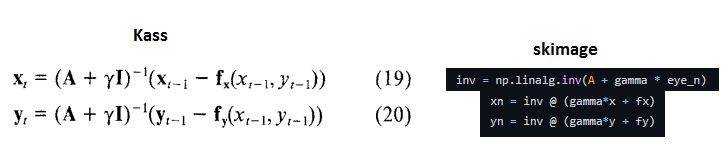
\includegraphics[width=1\textwidth]{gambar/skimage_vs_kass}
		\caption{Komparasi metode milik Kass dan \emph{skimage} }
		\label{Gambar:skimage_vs_kass}
	\end{figure}
	
\end{comment}


\section{Eksperimen}
\emph{Source code} eksperimen disimpan ke dalam repository yang dapat diakses di \url{https://github.com/m-rizki/skripsi} di bawah lisensi \emph{GNU General Public License v3.0}. Rancangan eksperimen deteksi keliling luka menggunakan \emph{snake} dan \emph{snake} yang ditambahkan interpolasi dilakukan dengan menjalankan program \emph{snake} hingga kurva akhir menutupi objek luka pada citra untuk semua data (populasi) yang tersedia. Proses ini memerlukan penyesuaian parameter algoritma \emph{snake} untuk setiap citra. Dari hasil yang didapatkan terdapat dua kategori hasil deteksi, yang pertama adalah kurva hasil deteksi berhasil menutupi luka (berhasil) dan kurva hasil deteksi tidak berhasil menutupi luka (gagal). Rincian parameter dan hasil dari proses deteksi tersedia di bagian \emph{lampiran C dan D}
\begin{figure}[H]
	\centering
	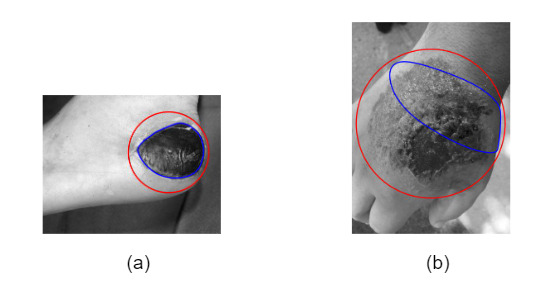
\includegraphics[width=0.5\textwidth]{gambar/result_good_bad}
	\caption{(a) Berhasil (b) Gagal}
	\label{Gambar:result_good_bad}
\end{figure}

Setelah hasil dikateorikan, langkah selanjutnya adalah mengidentifikasi area kurva hasil deteksi \emph{snake} yang berhasil dan di bandingkan terhadap area \emph{ground truth} untuk kemudian dihitung akurasinya menggunakan persamaan (\ref{val}). Rincian hasil dari proses ini tersedia di bagian \emph{lampiran C dan D}
\begin{figure}[H]
	\centering
	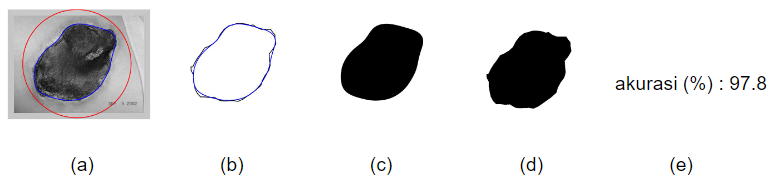
\includegraphics[width=0.8\textwidth]{gambar/result_val}
	\caption{(a) Hasil deteksi (b) Hasil deteksi \emph{overlay} dengan \emph{ground truth} (c) Area kurva akhir (d) Area \emph{ground truth} (e) Akurasi}
	\label{Gambar:result_val}
\end{figure}


\section{Analisa hasil}
Berikut analisa hasil setelah melakukan eksperimen terhadap populasi:
\begin{enumerate}
	\item Hasil dari deteksi keliling luka menggunakan \emph{snake} versi \emph{integer} kategori luka hitam menghasilkan 5 data (dari 24 data) yang kurva akhirnya berhasil menutupi luka dengan nilai akurasi rata-rata 84.2\%.
	\item Hasil dari deteksi keliling luka menggunakan \emph{snake} versi \emph{integer} kategori luka kuning menghasilkan 5 data (dari 15 data) yang kurva akhirnya berhasil menutupi luka dengan nilai akurasi rata-rata 76.14\%.
	\item Hasil dari deteksi keliling luka menggunakan \emph{snake} versi \emph{integer} kategori luka merah menghasilkan 2 data (dari 30 data) yang kurva akhirnya berhasil menutupi luka dengan nilai akurasi rata-rata 62.25\%.
	\item Hasil dari deteksi keliling luka menggunakan \emph{snake} versi \emph{intepolasi} kategori luka hitam menghasilkan 21 data (dari 24 data) yang kurva akhirnya berhasil menutupi luka dengan nilai akurasi rata-rata 87.6\%.
	\item Hasil dari deteksi keliling luka menggunakan \emph{snake} versi \emph{interpolasi} kategori luka kuning menghasilkan 11 data (dari 15 data) yang kurva akhirnya berhasil menutupi luka dengan nilai akurasi rata-rata 79.2\%.
	\item Hasil dari deteksi keliling luka menggunakan \emph{snake} versi \emph{interpolasi} kategori luka merah menghasilkan 12 data (dari 30 data) yang kurva akhirnya berhasil menutupi luka dengan nilai akurasi rata-rata 89.7\%.
	\item Hasil dari deteksi keliling luka menggunakan \emph{snake} versi \emph{integer} untuk semua kategori menghasilkan 12 data (dari 71 data) yang kurva akhirnya berhasil menutupi luka dengan nilai akurasi rata-rata 77.18\%.
	\item Hasil dari deteksi keliling luka menggunakan \emph{snake} versi \emph{integer} untuk semua kategori menghasilkan 44 data (dari 71 data) yang kurva akhirnya berhasil menutupi luka dengan nilai akurasi rata-rata 86.1\%.
\end{enumerate}

Sebagai tambahan, setelah dicek kembali ternyata terdapat kesalahan pada saat proses update iterasi kurva untuk metode \emph{snake} versi \emph{integer}. Sebelumnya penulis melakukan pembulatan terhadap kurva di luar iterasi dan di dalam iterasi, tetapi ternyata seharusnya penulis cukup melakukan proses pembulatan pada saat perhitungan \texttt{fx} dan \texttt{fy} di dalam iterasi saja sehingga kurva akhirnya tetap terdiri dari koordinat yang nilainya \emph{float}. Jika dibandingkan hasilnya sebagai berikut.
\begin{figure}[H]
	\centering
	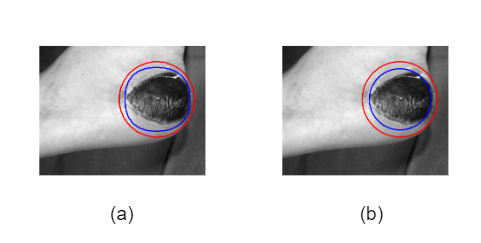
\includegraphics[width=1\textwidth]{gambar/compare_int}
	\caption{(a) Hasil \emph{snake} versi integer dengan pembulatan kurva di luar dan di dalam iterasi  (b) Hasil \emph{snake} versi integer dengan pembulatan kurva hanya di dalam iterasi}
	\label{Gambar:compare_int}
\end{figure}

\begin{figure}[H]
	\begin{lstlisting}[language=Python, basicstyle=\tiny]
		# potential force
		gy, gx = np.gradient(ext)
		
		xt = np.copy(x)
		yt = np.copy(y)
		
		max_num_iter=n
		for i in range(max_iter):
		fx = np.array([])
		fy = np.array([])
		
		for i in range(n):
		fx = np.append(fx, gx[np.round(yt[i]).astype(int)] [np.round(xt[i]).astype(int)] )
		fy = np.append(fy, gy[np.round(yt[i]).astype(int)] [np.round(xt[i]).astype(int)] )
		
		xn = np.dot(inv, xt + gamma * fx) # acton, ivins equation
		yn = np.dot(inv, yt + gamma * fy)
		
		xt = xn
		yt = yn
		
		snake_final = np.array([xt, yt]).T
	\end{lstlisting}
	\caption{\emph{source code} proses update iterasi kurva versi \emph{integer} dengan pembulatan kurva hanya di dalam iterasi}
	\label{code:snake_evol_int_2}
\end{figure}


\begin{comment}
	Sebagai catatan, penulis memasukan hasil inisialisasi kurva menggunakan metode manual, tetapi terkait kendala yang telah disebutkan di bagian \textbf{Inisialisasi kurva awal}, kurva akhir yang ditunjukkan hanya hasil dari proses deteksi menggunakan inisialisasi lingkaran.
\end{comment}

\begin{comment}
	content...

\subsection{Eksperimen kategori luka hitam}
Eksperimen pertama dilakukan terhadap data citra luka hitam, tabel yang disajikan memuat data hasil dari deteksi menggunakan metode \emph{snake} asli \emph{integer} dengan metode \emph{snake} yang ditambahkan interpolasi. Pertama mencatat parameter yang digunakan dalam proses deteksi, hasilnya sebagai berikut:
% anotasi integer
\begin{table}[H]
	\centering
	\caption{Anotasi parameter \emph{snake} versi \emph{integer} untuk kategori luka hitam }
	\label{hasil_1_0}
	\begin{tabular}{|c|c|c|c|c|c|c|c|c|c|}
		\hline
		\textbf{file} & \textbf{cr} & \textbf{cc} & \textbf{r} & \textbf{sigma}& \textbf{sample}& \textbf{alpha} & \textbf{beta} & \textbf{time step} & \textbf{max iter} \\
		\hline
		
		& &  &  & & & & & &\\
		luka\_hitam/2.jpg&120& 265& 85& 3.5& 100& 1& 10& 1& 100\\
		\hline
		luka\_hitam/5.jpg&160& 190& 115& 3.5& 100& 1& 10& 1& 100\\
		\hline
		luka\_hitam/7.jpg&55& 75& 35& 3.5& 50& 1& 10& 1& 25\\
		\hline
		luka\_hitam/15.jpg&153& 250& 151& 3.5& 200& 1& 10& 2& 100\\
		\hline
		luka\_hitam/26.jpg&195& 248& 193& 3.5& 200& 1& 10& 2& 100\\
		\hline
		luka\_hitam/28.jpg&120& 80& 60& 3.5& 200& 1& 10& 6& 50\\
		\hline
		luka\_hitam/37.jpg&110& 125& 90& 3.5& 200& 1& 10& 6& 100\\
		\hline
	\end{tabular}
\end{table}

%anotasi float
\begin{table}[H]
	\centering
	\caption{Anotasi parameter \emph{snake} versi interpolasi untuk kategori luka hitam}
	\label{hasil_1_1}
	\begin{tabular}{|c|c|c|c|c|c|c|c|c|c|}
		\hline
		\textbf{file} & \textbf{cr} & \textbf{cc} & \textbf{r} & \textbf{sigma}& \textbf{sample}& \textbf{alpha} & \textbf{beta} & \textbf{time step} & \textbf{max iter} \\
		\hline
		
		luka\_hitam/2.jpg&120& 265& 85& 3.5& 400& 0.015& 10& 0.001& 800\\
		\hline
		luka\_hitam/5.jpg&160& 190& 115& 3.5& 400& 0.015& 10& 0.001& 500\\
		\hline
		luka\_hitam/7.jpg&55& 75& 40& 3.5& 200& 0.015& 10& 0.001& 500\\
		\hline
		luka\_hitam/15.jpg&153& 250& 151& 3.5& 400& 0.015& 10& 0.001& 500\\
		\hline
		luka\_hitam/26.jpg&195& 248& 193& 3.5& 400& 0.015& 10& 0.001& 500\\
		\hline
		luka\_hitam/28.jpg&120& 80& 60& 3.5& 400& 0.015& 10& 0.001& 500\\
		\hline
		luka\_hitam/37.jpg&110& 125& 80& 3.5& 400& 0.015& 10& 0.001& 500\\
		\hline
	\end{tabular}
\end{table}

% Visualisasi hasil 
Yang kedua, memvisualisasikan hasil dari deteksi. Untuk kolom Hasil deteksi yang ditunjukkan adalah hasil dari proses deteksi menggunakan inisialisasi lingkaran, garis merah menunjukkan inisialisasi awal, garis biru menunjukkan kurva akhir.
\begin{table}[H]
	\centering
	\caption{Visualisasi hasil deteksi menggunakan \emph{snake} versi \emph{integer} untuk kategori luka hitam}
	\label{hasil_1_2}
	\begin{tabular}{|m{0.7in}|m{0.7in}|m{0.7in}|m{0.7in}|m{0.7in}|}
		\hline
		\textbf{Inisialisasi lingkaran} & \textbf{Inisialisasi manual} & \textbf{Energi Eksternal} & \textbf{Hasil deteksi} & \textbf{Hasil \& ground truth} \\
		\hline
		
		& &  &  &\\
		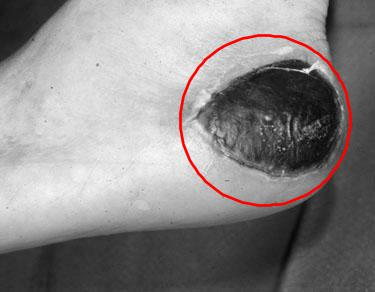
\includegraphics[width=0.7in]{dataset/dataset_3/luka_hitam/ready/2_integer_init.jpg} & 
		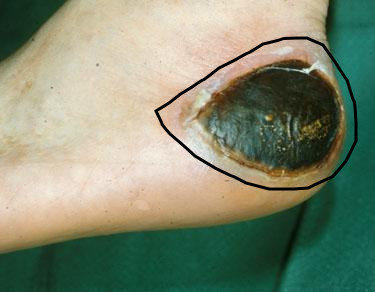
\includegraphics[width=0.7in]{dataset/dataset_3/luka_hitam/ready/2_manual.jpg}& 
		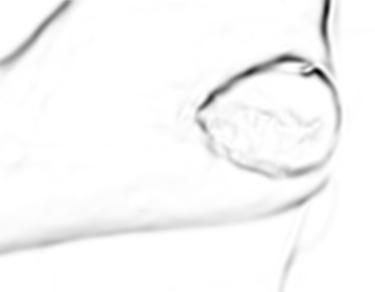
\includegraphics[width=0.7in]{dataset/dataset_3/luka_hitam/ready/2_integer_ext.jpg}&
		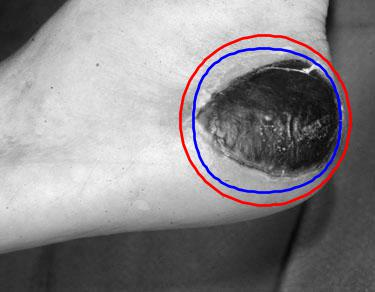
\includegraphics[width=0.7in]{dataset/dataset_3/luka_hitam/ready/2_integer_result.jpg}&
		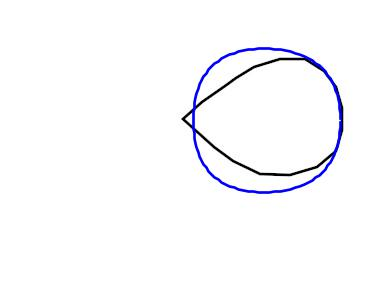
\includegraphics[width=0.7in]{dataset/dataset_3/luka_hitam/ready/2_gt_r_integer.jpg}\\
		\hline
		
		& &  &  &\\
		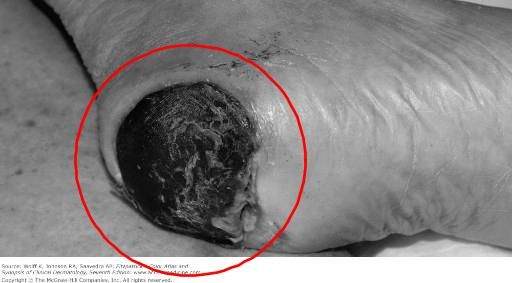
\includegraphics[width=0.7in]{dataset/dataset_3/luka_hitam/ready/5_integer_init.jpg} & 
		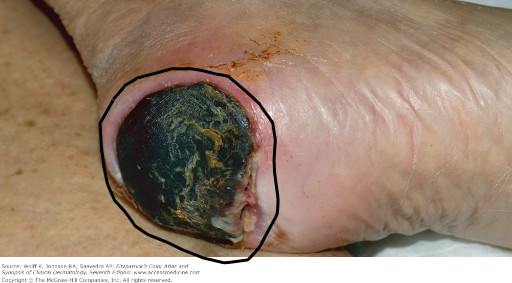
\includegraphics[width=0.7in]{dataset/dataset_3/luka_hitam/ready/5_manual.jpg}& 
		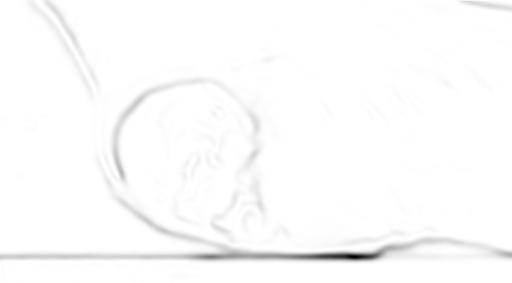
\includegraphics[width=0.7in]{dataset/dataset_3/luka_hitam/ready/5_integer_ext.jpg}&
		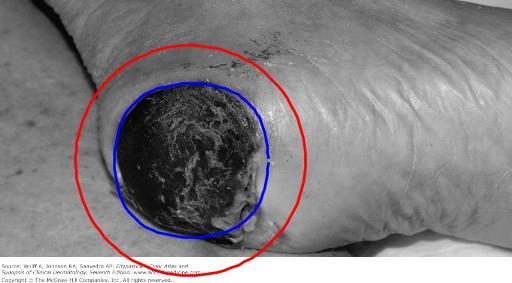
\includegraphics[width=0.7in]{dataset/dataset_3/luka_hitam/ready/5_integer_result.jpg}&
		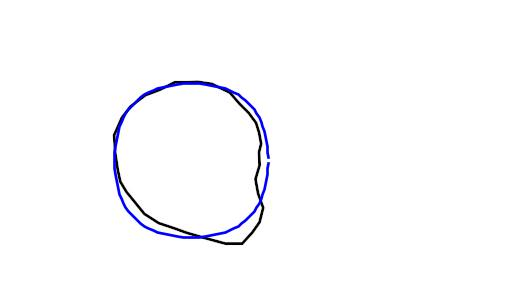
\includegraphics[width=0.7in]{dataset/dataset_3/luka_hitam/ready/5_gt_r_integer.jpg}\\
		\hline
		
		& &  &  &\\
		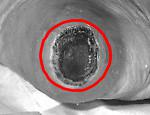
\includegraphics[width=0.7in]{dataset/dataset_3/luka_hitam/ready/7_integer_init.jpg} & 
		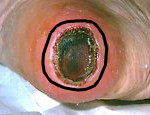
\includegraphics[width=0.7in]{dataset/dataset_3/luka_hitam/ready/7_manual.jpg}& 
		
\includegraphics[width=0.7in]{dataset/dataset_3/luka_hitam/ready/7_integer_ext.jpg}&
		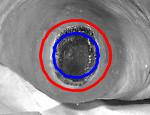
\includegraphics[width=0.7in]{dataset/dataset_3/luka_hitam/ready/7_integer_result.jpg}&
		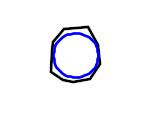
\includegraphics[width=0.7in]{dataset/dataset_3/luka_hitam/ready/7_gt_r_integer.jpg}\\
		\hline
		
		& &  &  &\\
		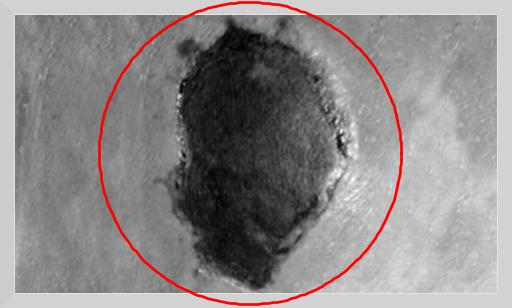
\includegraphics[width=0.7in]{dataset/dataset_3/luka_hitam/ready/15_integer_init.jpg} & 
		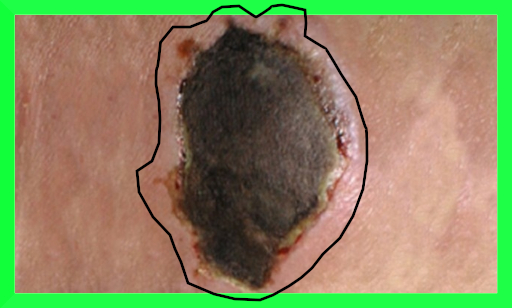
\includegraphics[width=0.7in]{dataset/dataset_3/luka_hitam/ready/15_manual.jpg}& 
		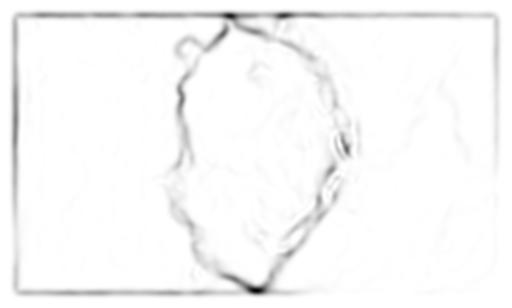
\includegraphics[width=0.7in]{dataset/dataset_3/luka_hitam/ready/15_integer_ext.jpg}&
		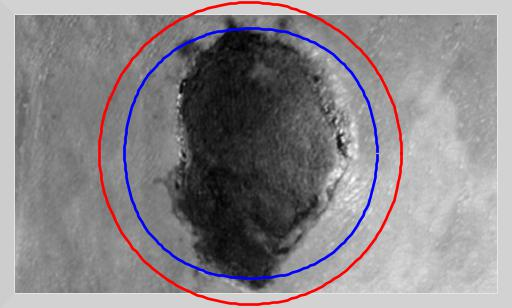
\includegraphics[width=0.7in]{dataset/dataset_3/luka_hitam/ready/15_integer_result.jpg}&
		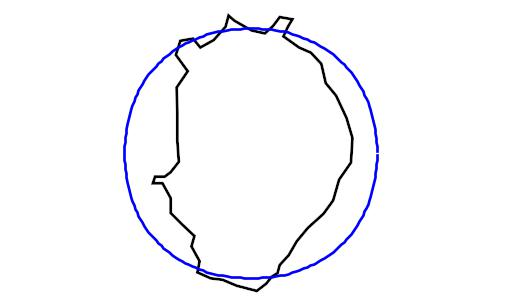
\includegraphics[width=0.7in]{dataset/dataset_3/luka_hitam/ready/15_gt_r_integer.jpg}\\
		\hline
		
		& &  &  &\\
		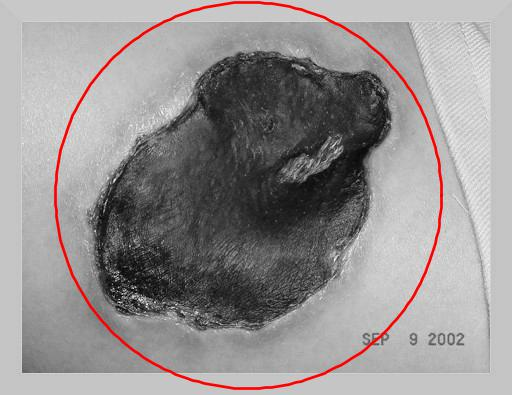
\includegraphics[width=0.7in]{dataset/dataset_3/luka_hitam/ready/26_integer_init.jpg} & 
		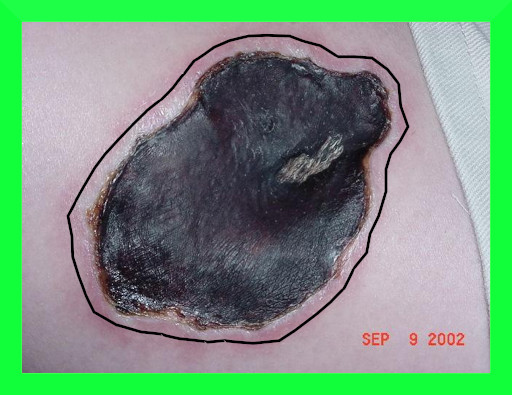
\includegraphics[width=0.7in]{dataset/dataset_3/luka_hitam/ready/26_manual.jpg}& 
		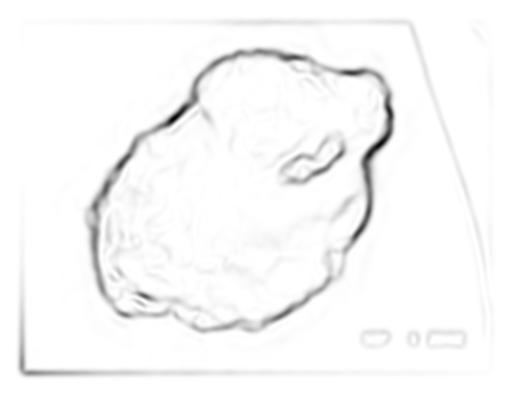
\includegraphics[width=0.7in]{dataset/dataset_3/luka_hitam/ready/26_integer_ext.jpg}&
		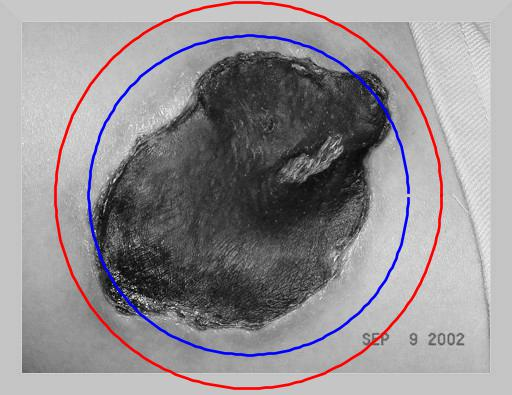
\includegraphics[width=0.7in]{dataset/dataset_3/luka_hitam/ready/26_integer_result.jpg}&
		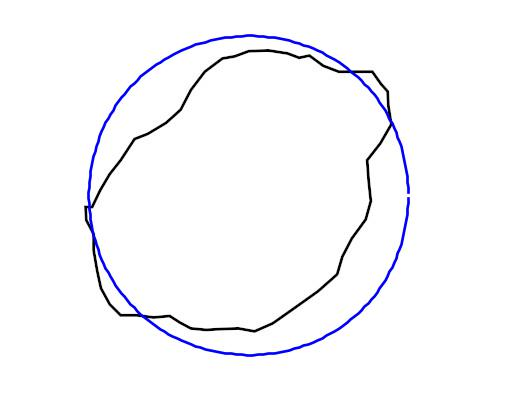
\includegraphics[width=0.7in]{dataset/dataset_3/luka_hitam/ready/26_gt_r_integer.jpg}\\
		\hline
		
		& &  &  &\\
		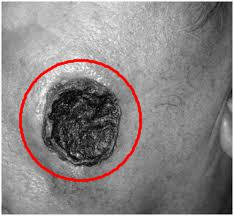
\includegraphics[width=0.7in]{dataset/dataset_3/luka_hitam/ready/28_integer_init.jpg} & 
		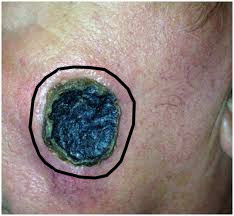
\includegraphics[width=0.7in]{dataset/dataset_3/luka_hitam/ready/28_manual.jpg}& 
		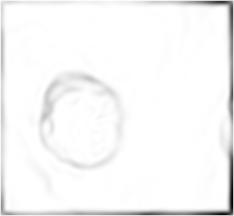
\includegraphics[width=0.7in]{dataset/dataset_3/luka_hitam/ready/28_integer_ext.jpg}&
		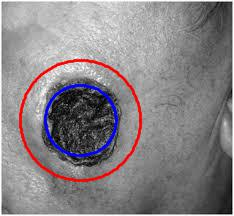
\includegraphics[width=0.7in]{dataset/dataset_3/luka_hitam/ready/28_integer_result.jpg}&
		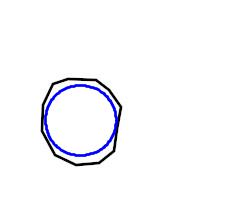
\includegraphics[width=0.7in]{dataset/dataset_3/luka_hitam/ready/28_gt_r_integer.jpg}\\
		\hline
		
		& &  &  &\\
		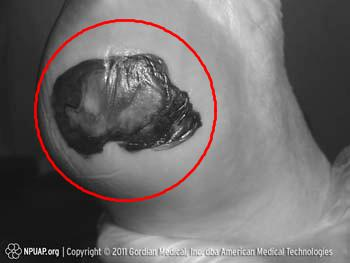
\includegraphics[width=0.7in]{dataset/dataset_3/luka_hitam/ready/37_integer_init.jpg} & 
		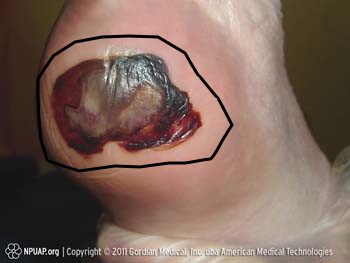
\includegraphics[width=0.7in]{dataset/dataset_3/luka_hitam/ready/37_manual.jpg}& 
		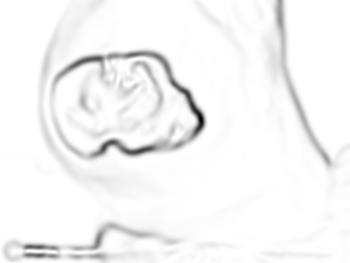
\includegraphics[width=0.7in]{dataset/dataset_3/luka_hitam/ready/37_integer_ext.jpg}&
		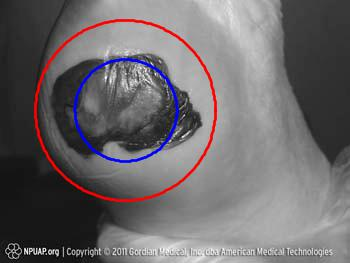
\includegraphics[width=0.7in]{dataset/dataset_3/luka_hitam/ready/37_integer_result.jpg}&
		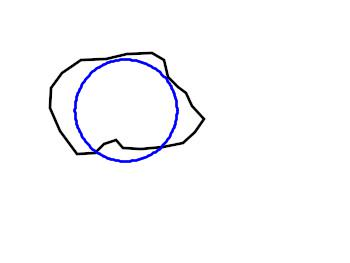
\includegraphics[width=0.7in]{dataset/dataset_3/luka_hitam/ready/37_gt_r_integer.jpg}\\
		\hline
	\end{tabular}
\end{table}

\begin{table}[H]
	\centering
	\caption{Visualisasi hasil deteksi menggunakan \emph{snake} versi interpolasi untuk kategori luka hitam}
	\label{hasil_1_3}
	\begin{tabular}{|m{0.7in}|m{0.7in}|m{0.7in}|m{0.7in}|m{0.7in}|}
		\hline
		\textbf{Inisialisasi lingkaran} & \textbf{Inisialisasi manual} & \textbf{Energi Eksternal} & \textbf{Hasil deteksi} & \textbf{Hasil \& ground truth} \\
		\hline
		& &  &  & \\
		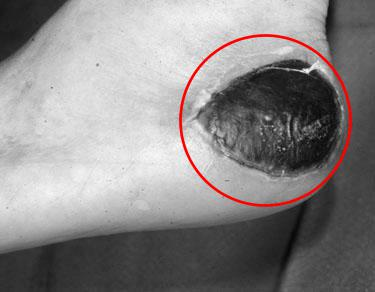
\includegraphics[width=0.7in]{dataset/dataset_3/luka_hitam/ready/2_interp_init.jpg} & 
		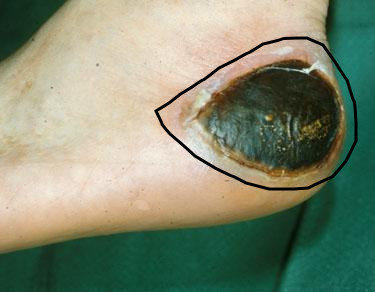
\includegraphics[width=0.7in]{dataset/dataset_3/luka_hitam/ready/2_manual.jpg}& 
		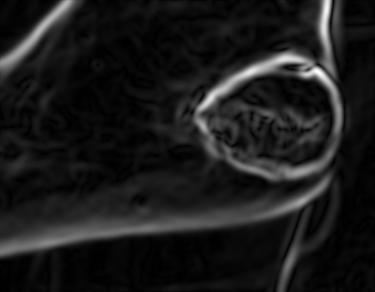
\includegraphics[width=0.7in]{dataset/dataset_3/luka_hitam/ready/2_interp_ext.jpg}&
		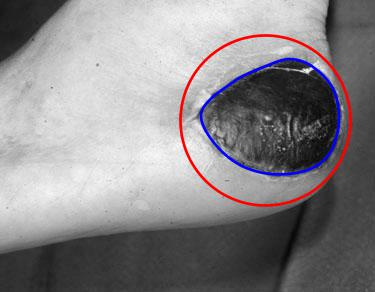
\includegraphics[width=0.7in]{dataset/dataset_3/luka_hitam/ready/2_interp_result.jpg}&
		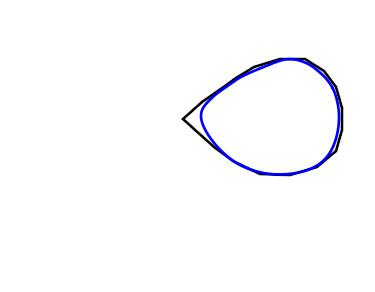
\includegraphics[width=0.7in]{dataset/dataset_3/luka_hitam/ready/2_gt_r.jpg}\\
		\hline
		
		& &  &  & \\
		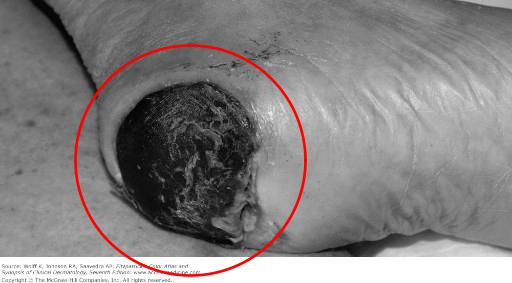
\includegraphics[width=0.7in]{dataset/dataset_3/luka_hitam/ready/5_interp_init.jpg} & 
		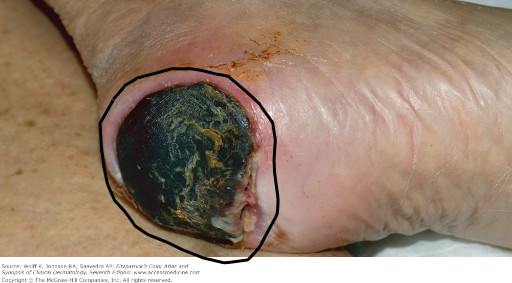
\includegraphics[width=0.7in]{dataset/dataset_3/luka_hitam/ready/5_manual.jpg}& 
		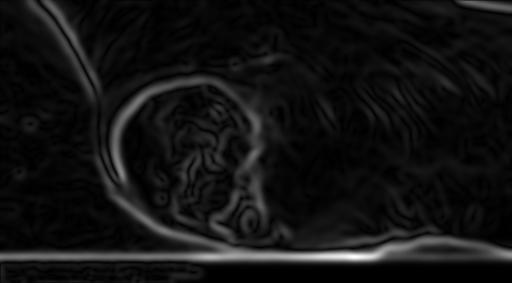
\includegraphics[width=0.7in]{dataset/dataset_3/luka_hitam/ready/5_interp_ext.jpg}&
		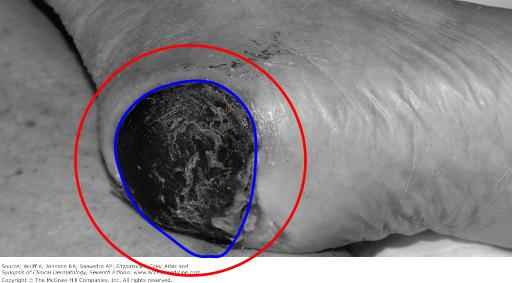
\includegraphics[width=0.7in]{dataset/dataset_3/luka_hitam/ready/5_interp_result.jpg}&
		\includegraphics[width=0.7in]{dataset/dataset_3/luka_hitam/ready/5_gt_r.jpg}\\
		\hline
		

		& &  &  & \\
		\includegraphics[width=0.7in]{dataset/dataset_3/luka_hitam/ready/7_interp_init.jpg} & 
		\includegraphics[width=0.7in]{dataset/dataset_3/luka_hitam/ready/7_manual.jpg}& 
		\includegraphics[width=0.7in]{dataset/dataset_3/luka_hitam/ready/7_interp_ext.jpg}&
		\includegraphics[width=0.7in]{dataset/dataset_3/luka_hitam/ready/7_interp_result.jpg}&
		\includegraphics[width=0.7in]{dataset/dataset_3/luka_hitam/ready/7_gt_r.jpg}\\
		\hline
		
		& &  &  & \\
		\includegraphics[width=0.7in]{dataset/dataset_3/luka_hitam/ready/15_interp_init.jpg} & 
		\includegraphics[width=0.7in]{dataset/dataset_3/luka_hitam/ready/15_manual.jpg}& 
		\includegraphics[width=0.7in]{dataset/dataset_3/luka_hitam/ready/15_interp_ext.jpg}&
		\includegraphics[width=0.7in]{dataset/dataset_3/luka_hitam/ready/15_interp_result.jpg}&
		\includegraphics[width=0.7in]{dataset/dataset_3/luka_hitam/ready/15_gt_r.jpg}\\
		\hline
		
		& &  &  & \\
		\includegraphics[width=0.7in]{dataset/dataset_3/luka_hitam/ready/26_interp_init.jpg} & 
		\includegraphics[width=0.7in]{dataset/dataset_3/luka_hitam/ready/26_manual.jpg}& 
		\includegraphics[width=0.7in]{dataset/dataset_3/luka_hitam/ready/26_interp_ext.jpg}&
		\includegraphics[width=0.7in]{dataset/dataset_3/luka_hitam/ready/26_interp_result.jpg}&
		\includegraphics[width=0.7in]{dataset/dataset_3/luka_hitam/ready/26_gt_r.jpg}\\
		\hline
		
		& &  &  & \\
		\includegraphics[width=0.7in]{dataset/dataset_3/luka_hitam/ready/28_interp_init.jpg} & 
		\includegraphics[width=0.7in]{dataset/dataset_3/luka_hitam/ready/28_manual.jpg}& 
		\includegraphics[width=0.7in]{dataset/dataset_3/luka_hitam/ready/28_interp_ext.jpg}&
		\includegraphics[width=0.7in]{dataset/dataset_3/luka_hitam/ready/28_interp_result.jpg}&
		\includegraphics[width=0.7in]{dataset/dataset_3/luka_hitam/ready/28_gt_r.jpg}\\
		\hline
		
		& &  &  & \\
		\includegraphics[width=0.7in]{dataset/dataset_3/luka_hitam/ready/37_interp_init.jpg} & 
		\includegraphics[width=0.7in]{dataset/dataset_3/luka_hitam/ready/37_manual.jpg}& 
		\includegraphics[width=0.7in]{dataset/dataset_3/luka_hitam/ready/37_interp_ext.jpg}&
		\includegraphics[width=0.7in]{dataset/dataset_3/luka_hitam/ready/37_interp_result.jpg}&
		\includegraphics[width=0.7in]{dataset/dataset_3/luka_hitam/ready/37_gt_r.jpg}\\
		\hline
	\end{tabular}
\end{table}

Yang ketiga adalah visualisasi area kurva akhir dengan \emph{ground truth} dan nilai validasi yang didapatkan dari selisih area kurva akhir dan area \emph{ground truth} dalam piksel.
\begin{table}[H]
	\centering
	\caption{Visualisasi area kurva akhir untuk kategori luka hitam}
	\label{hasil_1_4}
	\begin{tabular}{|m{0.7in}|m{0.7in}|m{0.7in}|m{0.7in}|m{0.7in}|}
		\hline
		\textbf{Area versi integer} & \textbf{Area versi interpolasi} & \textbf{Area ground truth} & selisih versi integer & \textbf{Selisih versi interpolasi} \\
		\hline
		& &  &  & \\
		\includegraphics[width=0.7in]{dataset/dataset_3/luka_hitam/ready/2_integer_r.jpg} & 
		\includegraphics[width=0.7in]{dataset/dataset_3/luka_hitam/ready/2_interp_r.jpg}& 
		\includegraphics[width=0.7in]{dataset/dataset_3/luka_hitam/ready/2_r.jpg}&
		5011&
		763\\
		
		& &  &  & \\
		\includegraphics[width=0.7in]{dataset/dataset_3/luka_hitam/ready/5_integer_r.jpg} & 
		\includegraphics[width=0.7in]{dataset/dataset_3/luka_hitam/ready/5_interp_r.jpg}& 
		\includegraphics[width=0.7in]{dataset/dataset_3/luka_hitam/ready/5_r.jpg}&
		1272&
		673\\
		
		& &  &  & \\
		\includegraphics[width=0.7in]{dataset/dataset_3/luka_hitam/ready/7_integer_r.jpg} & 
		\includegraphics[width=0.7in]{dataset/dataset_3/luka_hitam/ready/7_interp_r.jpg}& 
		\includegraphics[width=0.7in]{dataset/dataset_3/luka_hitam/ready/7_r.jpg}&
		574&
		334\\
		
		& &  &  & \\
		\includegraphics[width=0.7in]{dataset/dataset_3/luka_hitam/ready/15_integer_r.jpg} & 
		\includegraphics[width=0.7in]{dataset/dataset_3/luka_hitam/ready/15_interp_r.jpg}& 
		\includegraphics[width=0.7in]{dataset/dataset_3/luka_hitam/ready/15_r.jpg}&
		16947&
		1154\\
		
		& &  &  & \\
		\includegraphics[width=0.7in]{dataset/dataset_3/luka_hitam/ready/26_integer_r.jpg} & 
		\includegraphics[width=0.7in]{dataset/dataset_3/luka_hitam/ready/26_interp_r.jpg}& 
		\includegraphics[width=0.7in]{dataset/dataset_3/luka_hitam/ready/26_r.jpg}&
		20358&
		1514\\
		
		& &  &  & \\
		\includegraphics[width=0.7in]{dataset/dataset_3/luka_hitam/ready/28_integer_r.jpg} & 
		\includegraphics[width=0.7in]{dataset/dataset_3/luka_hitam/ready/28_interp_r.jpg}& 
		\includegraphics[width=0.7in]{dataset/dataset_3/luka_hitam/ready/28_r.jpg}&
		1593&
		347\\
		
		& &  &  & \\
		\includegraphics[width=0.7in]{dataset/dataset_3/luka_hitam/ready/37_integer_r.jpg} & 
		\includegraphics[width=0.7in]{dataset/dataset_3/luka_hitam/ready/37_interp_r.jpg}& 
		\includegraphics[width=0.7in]{dataset/dataset_3/luka_hitam/ready/37_r.jpg}&
		3148&
		714\\
		\hline
	\end{tabular}
\end{table}


%luka kuning
\subsection{Eksperimen kategori luka kuning}
Eksperimen pertama dilakukan terhadap data citra luka kuning, tabel yang disajikan memuat data hasil dari deteksi menggunakan metode \emph{snake} asli \emph{integer} dengan metode \emph{snake} yang ditambahkan interpolasi. Pertama mencatat parameter yang digunakan dalam proses deteksi, hasilnya sebagai berikut:
% anotasi integer
\begin{table}[H]
	\centering
	\caption{Anotasi parameter \emph{snake} versi \emph{integer} untuk kategori luka kuning }
	\label{hasil_2_0}
	\begin{tabular}{|c|c|c|c|c|c|c|c|c|c|}
		\hline
		\textbf{file} & \textbf{cr} & \textbf{cc} & \textbf{r} & \textbf{sigma}& \textbf{sample}& \textbf{alpha} & \textbf{beta} & \textbf{time step} & \textbf{max iter} \\
		\hline
		
		& &  &  & & & & & &\\
		luka\_kuning/10.jpg&155& 133& 115& 3.5& 100& 1& 10& 1& 100\\
		\hline
		luka\_kuning/16.jpg&135& 172& 130& 3.5& 100& 1& 10& 1& 100\\
		\hline
		luka\_kuning/19.jpg&60& 60& 50& 3.5& 100& 1& 10& 2& 100\\
		\hline
		luka\_kuning/23.jpg&170& 230& 160& 3.5& 100& 1& 10& 1& 100\\
		\hline
		luka\_kuning/25.jpg&145& 130& 55& 3.5& 100& 1& 10& 2& 100\\
		\hline
		luka\_kuning/34.jpg&185& 245& 130& 3.5& 100& 1& 10& 1& 100\\
		\hline
	\end{tabular}
\end{table}

%anotasi float
\begin{table}[H]
	\centering
	\caption{Anotasi parameter \emph{snake} versi interpolasi untuk kategori luka kuning}
	\label{hasil_2_1}
	\begin{tabular}{|c|c|c|c|c|c|c|c|c|c|}
		\hline
		\textbf{file} & \textbf{cr} & \textbf{cc} & \textbf{r} & \textbf{sigma}& \textbf{sample}& \textbf{alpha} & \textbf{beta} & \textbf{time step} & \textbf{max iter} \\
		\hline
		
		luka\_kuning/10.jpg&155& 133& 115& 3.5& 400& 0.015& 10& 0.001& 500\\
		\hline
		luka\_kuning/16.jpg&135& 172& 130& 3.5& 400& 0.015& 10& 0.001& 500\\
		\hline
		luka\_kuning/19.jpg&60& 60& 50& 3.5& 200& 0.015& 10& 0.001& 40\\
		\hline
		luka\_kuning/23.jpg&170& 230& 160& 3.5& 400& 0.015& 10& 0.001& 100\\
		\hline
		luka\_kuning/25.jpg&145& 130& 50& 3.5& 200& 0.015& 10& 0.001& 500\\
		\hline
		luka\_kuning/34.jpg&185& 245& 130& 3.5& 400& 0.015& 10& 0.001& 500\\
		\hline
	\end{tabular}
\end{table}

% Visualisasi hasil 
Yang kedua, memvisualisasikan hasil dari deteksi. Untuk kolom Hasil deteksi yang ditunjukkan adalah hasil dari proses deteksi menggunakan inisialisasi lingkaran, garis merah menunjukkan inisialisasi awal, garis biru menunjukkan kurva akhir.
\begin{table}[H]
	\centering
	\caption{Visualisasi hasil deteksi menggunakan \emph{snake} versi \emph{integer} untuk kategori luka kuning}
	\label{hasil_2_2}
	\begin{tabular}{|m{0.7in}|m{0.7in}|m{0.7in}|m{0.7in}|m{0.7in}|}
		\hline
		\textbf{Inisialisasi lingkaran} & \textbf{Inisialisasi manual} & \textbf{Energi Eksternal} & \textbf{Hasil deteksi} & \textbf{Hasil \& ground truth} \\
		\hline
		
		& &  &  &\\
		\includegraphics[width=0.7in]{dataset/dataset_3/luka_kuning/ready/10_integer_init.jpg} & 
		\includegraphics[width=0.7in]{dataset/dataset_3/luka_kuning/ready/10_manual.jpg}& 
		\includegraphics[width=0.7in]{dataset/dataset_3/luka_kuning/ready/10_integer_ext.jpg}&
		\includegraphics[width=0.7in]{dataset/dataset_3/luka_kuning/ready/10_integer_result.jpg}&
		\includegraphics[width=0.7in]{dataset/dataset_3/luka_kuning/ready/10_gt_r_integer.jpg}\\
		\hline
		
		& &  &  &\\
		\includegraphics[width=0.7in]{dataset/dataset_3/luka_kuning/ready/16_integer_init.jpg} & 
		\includegraphics[width=0.7in]{dataset/dataset_3/luka_kuning/ready/16_manual.jpg}& 
		\includegraphics[width=0.7in]{dataset/dataset_3/luka_kuning/ready/16_integer_ext.jpg}&
		\includegraphics[width=0.7in]{dataset/dataset_3/luka_kuning/ready/16_integer_result.jpg}&
		\includegraphics[width=0.7in]{dataset/dataset_3/luka_kuning/ready/16_gt_r_integer.jpg}\\
		\hline
		
		& &  &  &\\
		\includegraphics[width=0.7in]{dataset/dataset_3/luka_kuning/ready/19_integer_init.jpg} & 
		\includegraphics[width=0.7in]{dataset/dataset_3/luka_kuning/ready/19_manual.jpg}& 
		\includegraphics[width=0.7in]{dataset/dataset_3/luka_kuning/ready/19_integer_ext.jpg}&
		\includegraphics[width=0.7in]{dataset/dataset_3/luka_kuning/ready/19_integer_result.jpg}&
		\includegraphics[width=0.7in]{dataset/dataset_3/luka_kuning/ready/19_gt_r_integer.jpg}\\
		\hline
		
		& &  &  &\\
		\includegraphics[width=0.7in]{dataset/dataset_3/luka_kuning/ready/23_integer_init.jpg} & 
		\includegraphics[width=0.7in]{dataset/dataset_3/luka_kuning/ready/23_manual.jpg}& 
		\includegraphics[width=0.7in]{dataset/dataset_3/luka_kuning/ready/23_integer_ext.jpg}&
		\includegraphics[width=0.7in]{dataset/dataset_3/luka_kuning/ready/23_integer_result.jpg}&
		\includegraphics[width=0.7in]{dataset/dataset_3/luka_kuning/ready/23_gt_r_integer.jpg}\\
		\hline
		
		& &  &  &\\
		\includegraphics[width=0.7in]{dataset/dataset_3/luka_kuning/ready/25_integer_init.jpg} & 
		\includegraphics[width=0.7in]{dataset/dataset_3/luka_kuning/ready/25_manual.jpg}& 
		\includegraphics[width=0.7in]{dataset/dataset_3/luka_kuning/ready/25_integer_ext.jpg}&
		\includegraphics[width=0.7in]{dataset/dataset_3/luka_kuning/ready/25_integer_result.jpg}&
		\includegraphics[width=0.7in]{dataset/dataset_3/luka_kuning/ready/25_gt_r_integer.jpg}\\
		\hline
		
		& &  &  &\\
		\includegraphics[width=0.7in]{dataset/dataset_3/luka_kuning/ready/34_integer_init.jpg} & 
		\includegraphics[width=0.7in]{dataset/dataset_3/luka_kuning/ready/34_manual.jpg}& 
		\includegraphics[width=0.7in]{dataset/dataset_3/luka_kuning/ready/34_integer_ext.jpg}&
		\includegraphics[width=0.7in]{dataset/dataset_3/luka_kuning/ready/34_integer_result.jpg}&
		\includegraphics[width=0.7in]{dataset/dataset_3/luka_kuning/ready/34_gt_r_integer.jpg}\\
		\hline
	\end{tabular}
\end{table}

\begin{table}[H]
	\centering
	\caption{Visualisasi hasil deteksi menggunakan \emph{snake} versi interpolasi untuk kategori luka kuning}
	\label{hasil_2_3}
	\begin{tabular}{|m{0.7in}|m{0.7in}|m{0.7in}|m{0.7in}|m{0.7in}|}
		\hline
		\textbf{Inisialisasi lingkaran} & \textbf{Inisialisasi manual} & \textbf{Energi Eksternal} & \textbf{Hasil deteksi} & \textbf{Hasil \& ground truth} \\
		\hline
		& &  &  & \\
		\includegraphics[width=0.7in]{dataset/dataset_3/luka_kuning/ready/10_interp_init.jpg} & 
		\includegraphics[width=0.7in]{dataset/dataset_3/luka_kuning/ready/10_manual.jpg}& 
		\includegraphics[width=0.7in]{dataset/dataset_3/luka_kuning/ready/10_interp_ext.jpg}&
		\includegraphics[width=0.7in]{dataset/dataset_3/luka_kuning/ready/10_interp_result.jpg}&
		\includegraphics[width=0.7in]{dataset/dataset_3/luka_kuning/ready/10_gt_r.jpg}\\
		\hline
		
		& &  &  & \\
		\includegraphics[width=0.7in]{dataset/dataset_3/luka_kuning/ready/16_interp_init.jpg} & 
		\includegraphics[width=0.7in]{dataset/dataset_3/luka_kuning/ready/16_manual.jpg}& 
		\includegraphics[width=0.7in]{dataset/dataset_3/luka_kuning/ready/16_interp_ext.jpg}&
		\includegraphics[width=0.7in]{dataset/dataset_3/luka_kuning/ready/16_interp_result.jpg}&
		\includegraphics[width=0.7in]{dataset/dataset_3/luka_kuning/ready/16_gt_r.jpg}\\
		\hline
		
		& &  &  & \\
		\includegraphics[width=0.7in]{dataset/dataset_3/luka_kuning/ready/19_interp_init.jpg} & 
		\includegraphics[width=0.7in]{dataset/dataset_3/luka_kuning/ready/19_manual.jpg}& 
		\includegraphics[width=0.7in]{dataset/dataset_3/luka_kuning/ready/19_interp_ext.jpg}&
		\includegraphics[width=0.7in]{dataset/dataset_3/luka_kuning/ready/19_interp_result.jpg}&
		\includegraphics[width=0.7in]{dataset/dataset_3/luka_kuning/ready/19_gt_r.jpg}\\
		\hline
		
		& &  &  & \\
		\includegraphics[width=0.7in]{dataset/dataset_3/luka_kuning/ready/23_interp_init.jpg} & 
		\includegraphics[width=0.7in]{dataset/dataset_3/luka_kuning/ready/23_manual.jpg}& 
		\includegraphics[width=0.7in]{dataset/dataset_3/luka_kuning/ready/23_interp_ext.jpg}&
		\includegraphics[width=0.7in]{dataset/dataset_3/luka_kuning/ready/23_interp_result.jpg}&
		\includegraphics[width=0.7in]{dataset/dataset_3/luka_kuning/ready/23_gt_r.jpg}\\
		\hline
		
		& &  &  & \\
		\includegraphics[width=0.7in]{dataset/dataset_3/luka_kuning/ready/25_interp_init.jpg} & 
		\includegraphics[width=0.7in]{dataset/dataset_3/luka_kuning/ready/25_manual.jpg}& 
		\includegraphics[width=0.7in]{dataset/dataset_3/luka_kuning/ready/25_interp_ext.jpg}&
		\includegraphics[width=0.7in]{dataset/dataset_3/luka_kuning/ready/25_interp_result.jpg}&
		\includegraphics[width=0.7in]{dataset/dataset_3/luka_kuning/ready/25_gt_r.jpg}\\
		\hline
		
		& &  &  & \\
		\includegraphics[width=0.7in]{dataset/dataset_3/luka_kuning/ready/34_interp_init.jpg} & 
		\includegraphics[width=0.7in]{dataset/dataset_3/luka_kuning/ready/34_manual.jpg}& 
		\includegraphics[width=0.7in]{dataset/dataset_3/luka_kuning/ready/34_interp_ext.jpg}&
		\includegraphics[width=0.7in]{dataset/dataset_3/luka_kuning/ready/34_interp_result.jpg}&
		\includegraphics[width=0.7in]{dataset/dataset_3/luka_kuning/ready/34_gt_r.jpg}\\
		\hline
	\end{tabular}
\end{table}

Yang ketiga adalah visualisasi area kurva akhir dengan \emph{ground truth} dan nilai validasi yang didapatkan dari selisih area kurva akhir dan area \emph{ground truth} dalam piksel.
\begin{table}[H]
	\centering
	\caption{Visualisasi area kurva akhir untuk kategori luka kuning}
	\label{hasil_2_4}
	\begin{tabular}{|m{0.7in}|m{0.7in}|m{0.7in}|m{0.7in}|m{0.7in}|}
		\hline
		\textbf{Area versi integer} & \textbf{Area versi interpolasi} & \textbf{Area ground truth} & \textbf{selisih versi integer} & \textbf{Selisih versi interpolasi} \\
		\hline
		
		& &  &  & \\
		\includegraphics[width=0.7in]{dataset/dataset_3/luka_kuning/ready/10_integer_r.jpg} & 
		\includegraphics[width=0.7in]{dataset/dataset_3/luka_kuning/ready/10_interp_r.jpg}& 
		\includegraphics[width=0.7in]{dataset/dataset_3/luka_kuning/ready/10_r.jpg}&
		2036&
		12179\\
		\hline
		
		& &  &  & \\
		\includegraphics[width=0.7in]{dataset/dataset_3/luka_kuning/ready/16_integer_r.jpg} & 
		\includegraphics[width=0.7in]{dataset/dataset_3/luka_kuning/ready/16_interp_r.jpg}& 
		\includegraphics[width=0.7in]{dataset/dataset_3/luka_kuning/ready/16_r.jpg}&
		4121&
		16920\\
		\hline
		
		& &  &  & \\
		\includegraphics[width=0.7in]{dataset/dataset_3/luka_kuning/ready/19_integer_r.jpg} & 
		\includegraphics[width=0.7in]{dataset/dataset_3/luka_kuning/ready/19_interp_r.jpg}& 
		\includegraphics[width=0.7in]{dataset/dataset_3/luka_kuning/ready/19_r.jpg}&
		350&
		323\\
		\hline
		
		& &  &  & \\
		\includegraphics[width=0.7in]{dataset/dataset_3/luka_kuning/ready/23_integer_r.jpg} & 
		\includegraphics[width=0.7in]{dataset/dataset_3/luka_kuning/ready/23_interp_r.jpg}& 
		\includegraphics[width=0.7in]{dataset/dataset_3/luka_kuning/ready/23_r.jpg}&
		8201&
		1768\\
		\hline
		
		& &  &  & \\
		\includegraphics[width=0.7in]{dataset/dataset_3/luka_kuning/ready/25_integer_r.jpg} & 
		\includegraphics[width=0.7in]{dataset/dataset_3/luka_kuning/ready/25_interp_r.jpg}& 
		\includegraphics[width=0.7in]{dataset/dataset_3/luka_kuning/ready/25_r.jpg}&
		480&
		1505\\
		\hline
		
		& &  &  & \\
		\includegraphics[width=0.7in]{dataset/dataset_3/luka_kuning/ready/34_integer_r.jpg} & 
		\includegraphics[width=0.7in]{dataset/dataset_3/luka_kuning/ready/34_interp_r.jpg}& 
		\includegraphics[width=0.7in]{dataset/dataset_3/luka_kuning/ready/34_r.jpg}&
		233&
		7263\\
		\hline
	\end{tabular}
\end{table}


\subsection{Eksperimen kategori luka merah}
Eksperimen pertama dilakukan terhadap data citra luka luka merah, tabel yang disajikan memuat data hasil dari deteksi menggunakan metode \emph{snake} asli \emph{integer} dengan metode \emph{snake} yang ditambahkan interpolasi. Pertama mencatat parameter yang digunakan dalam proses deteksi, hasilnya sebagai berikut:
% anotasi integer
\begin{table}[H]
	\centering
	\caption{Anotasi parameter \emph{snake} versi \emph{integer} untuk kategori luka merah }
	\label{hasil_3_0}
	\begin{tabular}{|c|c|c|c|c|c|c|c|c|c|}
		\hline
		\textbf{file} & \textbf{cr} & \textbf{cc} & \textbf{r} & \textbf{sigma}& \textbf{sample}& \textbf{alpha} & \textbf{beta} & \textbf{time step} & \textbf{max iter} \\
		\hline
		
		& &  &  & & & & & &\\
		luka\_merah/2.jpg&270& 105& 100& 3.5& 100& 1& 10& 1& 100\\
		\hline
		
		& &  &  & & & & & &\\
		luka\_merah/3.jpg&255& 170& 100& 3.5& 100& 1& 10& 1& 100\\
		\hline
		
		& &  &  & & & & & &\\
		luka\_merah/8.jpg&220& 260& 140& 3.5& 100& 1& 10& 1& 100\\
		\hline
		
		& &  &  & & & & & &\\
		luka\_merah/9.jpg&236& 130& 70& 3.5& 100& 1& 10& 1& 100\\
		\hline
		
		& &  &  & & & & & &\\
		luka\_merah/11.jpg&190& 295& 100& 3.5& 100& 1& 10& 1& 100\\
		\hline
		
		& &  &  & & & & & &\\
		luka\_merah/14.jpg&255& 170& 100& 3.5& 100& 1& 10& 1& 100\\
		\hline
	\end{tabular}
\end{table}

%anotasi float
\begin{table}[H]
	\centering
	\caption{Anotasi parameter \emph{snake} versi interpolasi untuk kategori luka merah}
	\label{hasil_3_1}
	\begin{tabular}{|c|c|c|c|c|c|c|c|c|c|}
		\hline
		\textbf{file} & \textbf{cr} & \textbf{cc} & \textbf{r} & \textbf{sigma}& \textbf{sample}& \textbf{alpha} & \textbf{beta} & \textbf{time step} & \textbf{max iter} \\
		\hline
		
		luka\_merah/2.jpg&270&105&100 & 3.5& 400& 0.015& 10& 0.001& 500\\
		\hline
		luka\_merah/3.jpg&255&170 &100 & 3.5& 400& 0.015& 10& 0.001& 500\\
		\hline
		luka\_merah/8.jpg&220&260 &140 & 3.5& 400& 0.015& 10& 0.001& 500\\
		\hline
		luka\_merah/9.jpg&236&130 &70 & 3.5& 400& 0.015& 10& 0.001& 500\\
		\hline
		luka\_merah/11.jpg&190&295 &170 & 3.5& 400& 0.015& 10& 0.001& 500\\
		\hline
		luka\_merah/14.jpg&180&263 &175 & 3.5& 400& 0.015& 10& 0.001& 500\\
		\hline
	\end{tabular}
\end{table}

% Visualisasi hasil 
Yang kedua, memvisualisasikan hasil dari deteksi. Untuk kolom Hasil deteksi yang ditunjukkan adalah hasil dari proses deteksi menggunakan inisialisasi lingkaran, garis merah menunjukkan inisialisasi awal, garis biru menunjukkan kurva akhir.
\begin{table}[H]
	\centering
	\caption{Visualisasi hasil deteksi menggunakan \emph{snake} versi \emph{integer} untuk kategori luka merah}
	\label{hasil_3_2}
	\begin{tabular}{|m{0.7in}|m{0.7in}|m{0.7in}|m{0.7in}|m{0.7in}|}
		\hline
		\textbf{Inisialisasi lingkaran} & \textbf{Inisialisasi manual} & \textbf{Energi Eksternal} & \textbf{Hasil deteksi} & \textbf{Hasil \& ground truth} \\
		\hline
		
		& &  &  &\\
		\includegraphics[width=0.7in]{dataset/dataset_3/luka_merah/ready/2_integer_init.jpg} & 
		\includegraphics[width=0.7in]{dataset/dataset_3/luka_merah/ready/2_manual.jpg}& 
		\includegraphics[width=0.7in]{dataset/dataset_3/luka_merah/ready/2_integer_ext.jpg}&
		\includegraphics[width=0.7in]{dataset/dataset_3/luka_merah/ready/2_integer_result.jpg}&
		\includegraphics[width=0.7in]{dataset/dataset_3/luka_merah/ready/2_gt_r_integer.jpg}\\
		\hline
		
		& &  &  &\\
		\includegraphics[width=0.7in]{dataset/dataset_3/luka_merah/ready/3_integer_init.jpg} & 
		\includegraphics[width=0.7in]{dataset/dataset_3/luka_merah/ready/3_manual.jpg}& 
		\includegraphics[width=0.7in]{dataset/dataset_3/luka_merah/ready/3_integer_ext.jpg}&
		\includegraphics[width=0.7in]{dataset/dataset_3/luka_merah/ready/3_integer_result.jpg}&
		\includegraphics[width=0.7in]{dataset/dataset_3/luka_merah/ready/3_gt_r_integer.jpg}\\
		\hline
		
		& &  &  &\\
		\includegraphics[width=0.7in]{dataset/dataset_3/luka_merah/ready/8_integer_init.jpg} & 
		\includegraphics[width=0.7in]{dataset/dataset_3/luka_merah/ready/8_manual.jpg}& 
		\includegraphics[width=0.7in]{dataset/dataset_3/luka_merah/ready/8_integer_ext.jpg}&
		\includegraphics[width=0.7in]{dataset/dataset_3/luka_merah/ready/8_integer_result.jpg}&
		\includegraphics[width=0.7in]{dataset/dataset_3/luka_merah/ready/8_gt_r_integer.jpg}\\
		\hline
		
		& &  &  &\\
		\includegraphics[width=0.7in]{dataset/dataset_3/luka_merah/ready/9_integer_init.jpg} & 
		\includegraphics[width=0.7in]{dataset/dataset_3/luka_merah/ready/9_manual.jpg}& 
		\includegraphics[width=0.7in]{dataset/dataset_3/luka_merah/ready/9_integer_ext.jpg}&
		\includegraphics[width=0.7in]{dataset/dataset_3/luka_merah/ready/9_integer_result.jpg}&
		\includegraphics[width=0.7in]{dataset/dataset_3/luka_merah/ready/9_gt_r_integer.jpg}\\
		\hline
		
		& &  &  &\\
		\includegraphics[width=0.7in]{dataset/dataset_3/luka_merah/ready/11_integer_init.jpg} & 
		\includegraphics[width=0.7in]{dataset/dataset_3/luka_merah/ready/11_manual.jpg}& 
		\includegraphics[width=0.7in]{dataset/dataset_3/luka_merah/ready/11_integer_ext.jpg}&
		\includegraphics[width=0.7in]{dataset/dataset_3/luka_merah/ready/11_integer_result.jpg}&
		\includegraphics[width=0.7in]{dataset/dataset_3/luka_merah/ready/11_gt_r_integer.jpg}\\
		\hline
		
		& &  &  &\\
		\includegraphics[width=0.7in]{dataset/dataset_3/luka_merah/ready/14_integer_init.jpg} & 
		\includegraphics[width=0.7in]{dataset/dataset_3/luka_merah/ready/14_manual.jpg}& 
		\includegraphics[width=0.7in]{dataset/dataset_3/luka_merah/ready/14_integer_ext.jpg}&
		\includegraphics[width=0.7in]{dataset/dataset_3/luka_merah/ready/14_integer_result.jpg}&
		\includegraphics[width=0.7in]{dataset/dataset_3/luka_merah/ready/14_gt_r_integer.jpg}\\
		\hline
	\end{tabular}
\end{table}

\begin{table}[H]
	\centering
	\caption{Visualisasi hasil deteksi menggunakan \emph{snake} versi interpolasi untuk kategori luka merah}
	\label{hasil_3_3}
	\begin{tabular}{|m{0.7in}|m{0.7in}|m{0.7in}|m{0.7in}|m{0.7in}|}
		\hline
		\textbf{Inisialisasi lingkaran} & \textbf{Inisialisasi manual} & \textbf{Energi Eksternal} & \textbf{Hasil deteksi} & \textbf{Hasil \& ground truth} \\
		\hline
		& &  &  & \\
		\includegraphics[width=0.7in]{dataset/dataset_3/luka_merah/ready/2_interp_init.jpg} & 
		\includegraphics[width=0.7in]{dataset/dataset_3/luka_merah/ready/2_manual.jpg}& 
		\includegraphics[width=0.7in]{dataset/dataset_3/luka_merah/ready/2_interp_ext.jpg}&
		\includegraphics[width=0.7in]{dataset/dataset_3/luka_merah/ready/2_interp_result.jpg}&
		\includegraphics[width=0.7in]{dataset/dataset_3/luka_merah/ready/2_gt_r.jpg}\\
		\hline
		
		& &  &  & \\
		\includegraphics[width=0.7in]{dataset/dataset_3/luka_merah/ready/3_interp_init.jpg} & 
		\includegraphics[width=0.7in]{dataset/dataset_3/luka_merah/ready/3_manual.jpg}& 
		\includegraphics[width=0.7in]{dataset/dataset_3/luka_merah/ready/3_interp_ext.jpg}&
		\includegraphics[width=0.7in]{dataset/dataset_3/luka_merah/ready/3_interp_result.jpg}&
		\includegraphics[width=0.7in]{dataset/dataset_3/luka_merah/ready/3_gt_r.jpg}\\
		\hline
		
		& &  &  & \\
		\includegraphics[width=0.7in]{dataset/dataset_3/luka_merah/ready/8_interp_init.jpg} & 
		\includegraphics[width=0.7in]{dataset/dataset_3/luka_merah/ready/8_manual.jpg}& 
		\includegraphics[width=0.7in]{dataset/dataset_3/luka_merah/ready/8_interp_ext.jpg}&
		\includegraphics[width=0.7in]{dataset/dataset_3/luka_merah/ready/8_interp_result.jpg}&
		\includegraphics[width=0.7in]{dataset/dataset_3/luka_merah/ready/8_gt_r.jpg}\\
		\hline
		
		& &  &  & \\
		\includegraphics[width=0.7in]{dataset/dataset_3/luka_merah/ready/9_interp_init.jpg} & 
		\includegraphics[width=0.7in]{dataset/dataset_3/luka_merah/ready/9_manual.jpg}& 
		\includegraphics[width=0.7in]{dataset/dataset_3/luka_merah/ready/9_interp_ext.jpg}&
		\includegraphics[width=0.7in]{dataset/dataset_3/luka_merah/ready/9_interp_result.jpg}&
		\includegraphics[width=0.7in]{dataset/dataset_3/luka_merah/ready/9_gt_r.jpg}\\
		\hline
		
		& &  &  & \\
		\includegraphics[width=0.7in]{dataset/dataset_3/luka_merah/ready/11_interp_init.jpg} & 
		\includegraphics[width=0.7in]{dataset/dataset_3/luka_merah/ready/11_manual.jpg}& 
		\includegraphics[width=0.7in]{dataset/dataset_3/luka_merah/ready/11_interp_ext.jpg}&
		\includegraphics[width=0.7in]{dataset/dataset_3/luka_merah/ready/11_interp_result.jpg}&
		\includegraphics[width=0.7in]{dataset/dataset_3/luka_merah/ready/11_gt_r.jpg}\\
		\hline
		
		& &  &  & \\
		\includegraphics[width=0.7in]{dataset/dataset_3/luka_merah/ready/14_interp_init.jpg} & 
		\includegraphics[width=0.7in]{dataset/dataset_3/luka_merah/ready/14_manual.jpg}& 
		\includegraphics[width=0.7in]{dataset/dataset_3/luka_merah/ready/14_interp_ext.jpg}&
		\includegraphics[width=0.7in]{dataset/dataset_3/luka_merah/ready/14_interp_result.jpg}&
		\includegraphics[width=0.7in]{dataset/dataset_3/luka_merah/ready/14_gt_r.jpg}\\
		\hline
		
	\end{tabular}
\end{table}

Yang ketiga adalah visualisasi area kurva akhir dengan \emph{ground truth} dan nilai validasi yang didapatkan dari selisih area kurva akhir dan area \emph{ground truth} dalam piksel.
\begin{table}[H]
	\centering
	\caption{Visualisasi area kurva akhir untuk kategori luka merah}
	\label{hasil_3_4}
	\begin{tabular}{|m{0.7in}|m{0.7in}|m{0.7in}|m{0.7in}|m{0.7in}|}
		\hline
		\textbf{Area versi integer} & \textbf{Area versi interpolasi} & \textbf{Area ground truth} & \textbf{selisih versi integer} & \textbf{Selisih versi interpolasi} \\
		\hline
		
		& &  &  & \\
		\includegraphics[width=0.7in]{dataset/dataset_3/luka_merah/ready/2_integer_r.jpg} & 
		\includegraphics[width=0.7in]{dataset/dataset_3/luka_merah/ready/2_interp_r.jpg}& 
		\includegraphics[width=0.7in]{dataset/dataset_3/luka_merah/ready/2_r.jpg}&
		17489&
		14760\\
		\hline
		
		& &  &  & \\
		\includegraphics[width=0.7in]{dataset/dataset_3/luka_merah/ready/3_integer_r.jpg} & 
		\includegraphics[width=0.7in]{dataset/dataset_3/luka_merah/ready/3_interp_r.jpg}& 
		\includegraphics[width=0.7in]{dataset/dataset_3/luka_merah/ready/3_r.jpg}&
		19400&
		3071\\
		\hline
		
		& &  &  & \\
		\includegraphics[width=0.7in]{dataset/dataset_3/luka_merah/ready/8_integer_r.jpg} & 
		\includegraphics[width=0.7in]{dataset/dataset_3/luka_merah/ready/8_interp_r.jpg}& 
		\includegraphics[width=0.7in]{dataset/dataset_3/luka_merah/ready/8_r.jpg}&
		40325&
		27626\\
		\hline
		
		& &  &  & \\
		\includegraphics[width=0.7in]{dataset/dataset_3/luka_merah/ready/9_integer_r.jpg} & 
		\includegraphics[width=0.7in]{dataset/dataset_3/luka_merah/ready/9_interp_r.jpg}& 
		\includegraphics[width=0.7in]{dataset/dataset_3/luka_merah/ready/9_r.jpg}&
		5965&
		7379\\
		\hline
		
		& &  &  & \\
		\includegraphics[width=0.7in]{dataset/dataset_3/luka_merah/ready/11_integer_r.jpg} & 
		\includegraphics[width=0.7in]{dataset/dataset_3/luka_merah/ready/11_interp_r.jpg}& 
		\includegraphics[width=0.7in]{dataset/dataset_3/luka_merah/ready/11_r.jpg}&
		7110&
		24345\\
		\hline
		
		& &  &  & \\
		\includegraphics[width=0.7in]{dataset/dataset_3/luka_merah/ready/14_integer_r.jpg} & 
		\includegraphics[width=0.7in]{dataset/dataset_3/luka_merah/ready/14_interp_r.jpg}& 
		\includegraphics[width=0.7in]{dataset/dataset_3/luka_merah/ready/14_r.jpg}&
		6863&
		12533\\
		\hline
		
	\end{tabular}
\end{table}

\end{comment}


% Baris ini digunakan untuk membantu dalam melakukan sitasi
% Karena diapit dengan comment, maka baris ini akan diabaikan
% oleh compiler LaTeX.
\begin{comment}
\bibliography{daftar-pustaka}
\end{comment}